\documentclass[final,3p]{CSP}
\usepackage{amssymb}
\usepackage{changepage}
\usepackage{float}
\usepackage{hyperref}
\usepackage{url}
\usepackage{afterpage}
\usepackage{natbib}
\usepackage{setspace}
\usepackage{fancyhdr}
\pagestyle{fancy}
\fancyhf{}

\def\Student{Ashish Sehrawat}
\def\Title{MONOGRAPH}
\def\Prog{Doctorado en Ciencias (F\'{i}sica) }
\def\Dept{Departamento de Investigac\'{i}on en Fis\'{i}ca}
\def\Director{Dr. Jos\'{e} Feliciano Ben\'{i}tez Rubio}
\def\Universidad{\it Universidad de Sonora}
\def\ProjectTitle{ Measurement of .. }
\def\ResearchLine{Astrof\'{i}sica, Cosmolog\'{i}a y F\'{i}sica de Part\'{i}culas}


\newcommand{\SubItem}[1]{
    {\setlength\itemindent{15pt} \item[-] #1}
}


%%header and footer
\lhead{\Student / \Prog }
\rhead{\Title}
\lfoot{\Dept}
\rfoot{Page \thepage}
\setlength{\headsep}{0.2in}
\renewcommand{\footrulewidth}{0.4pt}% default is 0pt


\begin{document}

%%%%Cover page
\begin{titlepage}
  \centering
  \hspace{0pt}
  \vfill
        {\scshape\Large \Title \par}

	\vspace{2cm}
        \begin{adjustwidth}{2cm}{2cm}{
            TITLE:\par
            {\large \ProjectTitle \par}
          }
        \end{adjustwidth}

%	\vspace{0.5cm}
%        \begin{adjustwidth}{2cm}{2cm}{
%            RESEARCH LINE: \par
%            \ResearchLine \par}
%        \end{adjustwidth}

        
        \vspace{4cm}
        {\underline{\hspace{8cm}}\par}
	{\scshape\large \Student \par}
        {PhD. Student\par}

        \vspace{1cm}
        {\underline{\hspace{8cm}}\par}
	{\Director \par}
        {Thesis Director\par}

        \vspace{1cm}
        {\Prog \par}
        {\Dept \par}
        {\Universidad \par}

        \vspace{4cm}
	{\today}

\hspace{0pt}
\vfill

\end{titlepage}


%%%%% white page for print out
\shipout\null


%%%% Title and Abstract Page
\newpage
\hspace{2pt}
%\vfill

\begin{adjustwidth}{1cm}{1cm}

  \begin{center}
    {\Large \ProjectTitle \par}
    \vspace{0.5cm}

    {\Student \par}
    {\Universidad \par}  
    \vspace{1cm}
    
    {\itshape\textbf{Abstract}\par}
     \vspace{0.7 cm}
        
    \end{center}  

 
    \onehalfspacing
    This research project proposes ...

\end{adjustwidth}

\hspace{2pt}
%\vfill
\vspace{1 cm}


%%%%%% Begin the body
%\newpage
\section{INTRODUCTION}


\onehalfspacing The standard model (SM) of particle physics is so far the best theoretical model to describe the interaction of elementary 
particles using three of the four fundamental forces of nature which are electromagnetic force, strong nuclear force and the 
weak nuclear force. Gravitational force is neglected as the strength of this force is very weak at the scales over which 
elementary particle interact with each other. The standard model (SM) of particle physics is divided into two categories, 
bosonic sector and fermionic sector. Bosonic sector contain particles called bosons which mediate the fundamental forces of 
nature and the fermionic sector contain particles called fermions which make up all the matter in our universe. SM has three 
generations of matter (fermions) particles. The first generation of fermions consists of up (u) quark, down (d) quark, electron 
and electron neutrino, second generation consist of charm (c) quark, strange (s) quark, muon and muon neutrino and the third 
generation of matter particles has top (t) quark, bottom (b) quark, tau and tau neutrino. The bosonic sector consist of gauge 
bosons like gluon, photon, $W^{\pm}$, $Z^0$ which mediate strong nuclear force, electromagnetic force and weak nuclear force respectively. There is one more particle in the standard model called the Higgs Boson which gives mass to SM particles via electroweak symmetry breaking mechanism \cite{Chatrchyan:2012xdj}. All the standard model particles are shown in Figure 1. Higgs boson can be produced at the particle colliders like the Large Hadron Collider (LHC) in Geneva, Switzerland.


LHC during the first run in 2011 and 2012 reached a peak instantaneous luminosity of 7.7 $\times$ $10^{33}$ $cm^{-2}s^{-1}$ which was more than 75$\%$ of its design luminosity and delivered an integrated luminosity of about 25 $fb^{-1}$ to each ATLAS and CMS.
 The LHC will deliver about 300 $fb^{-1}$ by 2024 \cite{collaborations2019report}.
The goal of subsequently run of LHC has been to obtain datasets at higher values of luminosities for precision measurements of the properties of Higgs boson, in order to test the Standard Model pattern of couplings to elementary particles.
In order to minimize the machine downtimes and maximize the productive use of the LHC for physics, the replacement of the inner triplet magnets (the one responsible to squeeze the beam at collision) and  of  all  hardware  changes  needed  to  enable  an  ambitious  luminosity  upgrade  will  take  place in parallel during one shutdown, at around 2023-25 (LS3), with some of the modification anticipated in 2019-2020 (LS2).
This new phase of the LHC life has been named as High Luminosity LHC (HL-LHC) and has the scope of attaining the astonishing threshold of 3000 $fb^{-1}$ by the year 2036 as shown in Figure~\ref{figure6}.
Figure~\ref{figureKappas} shows a summary of the current measurements of the Higgs coupling parameters with the LHC Run 1 dataset (2011,2012)  using ggF, VBF, VH, and ${t\bar{t}H}$ production modes \cite{Tanabashi:2018oca}.


\begin{figure}[H]
  \centering
  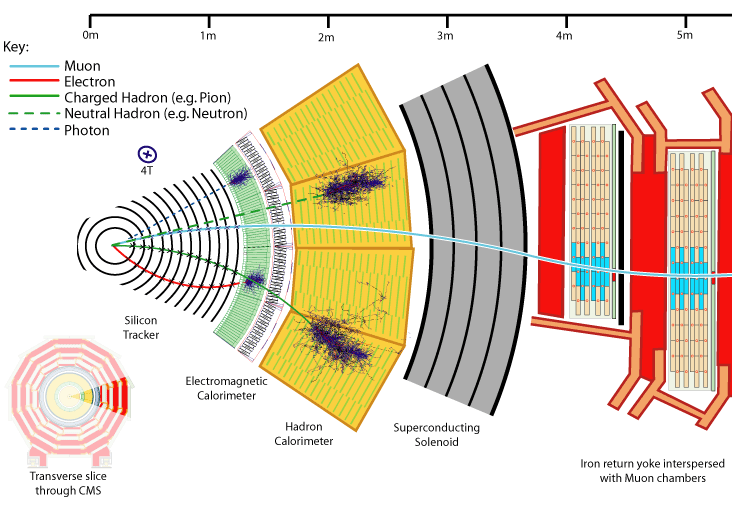
\includegraphics[width=0.6\columnwidth]{./cms12.png}
  \caption{Transverse view of the CMS detector showing the silicon tracker, electromagnetic calorimeter, hadron calorimeter, superconducting solenoid and muon chambers \cite{Chatrchyan:2008aa}.}
  \label{figure5}
\end{figure}


\section{PCC method}
\onehalfspacing



\section{vdM Calibration}
\onehalfspacing



\section{Backgrounds}
\onehalfspacing


\section{Systematics}
\onehalfspacing


\section{Results}
\onehalfspacing


\section{Conclusions}
\onehalfspacing



\cleardoublepage
\onehalfspacing
\bibliographystyle{unsrt}
\bibliography{paper}

\end{document}

